\documentclass[conference]{IEEEtran}
% Compiles with pdfLaTeX + BibTeX (Overleaf default). Standard packages only.
\IEEEoverridecommandlockouts
\usepackage[T1]{fontenc}
\usepackage{cite}
\usepackage{amsmath,amssymb}
\usepackage{graphicx}
\usepackage{booktabs}
\usepackage{tabularx}
\usepackage{array}
\usepackage{multirow}
\usepackage{xcolor}
\usepackage{url}
\usepackage{algorithm}
\usepackage{algpseudocode}
\usepackage{tikz}
\usetikzlibrary{positioning,arrows.meta,fit,backgrounds,calc,shapes.geometric}
\usepackage[hidelinks]{hyperref}
\def\UrlBreaks{\do\/\do-\do.\do_}

\newcolumntype{L}{>{\raggedright\arraybackslash}X}
\newcolumntype{P}[1]{>{\raggedright\arraybackslash}p{#1}}
\newcommand{\code}[1]{\texttt{\small #1}}
\renewcommand{\algorithmicrequire}{\textbf{Input:}}
\renewcommand{\algorithmicensure}{\textbf{Output:}}

\begin{document}

\title{Zero-Trust Multi-Cloud Chunked Storage Framework with Privacy-Aware Audit Logging}

\author{
\IEEEauthorblockN{Vaibhav Sharma}
\IEEEauthorblockA{USN: 23BDS066\\
\textit{Indian Institute of}\\\textit{Information Technology}\\\textit{Dharwad, India}}
\and
\IEEEauthorblockN{Shivansh Shukla}
\IEEEauthorblockA{USN: 23BDS054\\
\textit{Indian Institute of}\\\textit{Information Technology}\\\textit{Dharwad, India}}
\and
\IEEEauthorblockN{Kishlay Singh}
\IEEEauthorblockA{USN: 23BCS066\\
\textit{Indian Institute of}\\\textit{Information Technology}\\\textit{Dharwad, India}}
\and
\IEEEauthorblockN{Dhanraj Matke}
\IEEEauthorblockA{USN: 23BCS042\\
\textit{Indian Institute of}\\\textit{Information Technology}\\\textit{Dharwad, India}}
}

\maketitle

% NUMBERS: abstract quotes 1,273 passing tests, the cost ratio and success counts from analysis/data (Section~\ref{sec:stats}), 108 security tests, 17 attack scenarios,
% 46/46 demo checks, 6 + 17 findings, 0.54 s audit verification (see Section VI).
\begin{abstract}
In the 2024 Snowflake customer-instance campaign attributed to UNC5537, attackers used passwords stolen by infostealer malware to sign in to accounts without multi-factor authentication or network allow lists and then exported data through ordinary platform functions. Encryption was working throughout; it simply could not stop an authenticated session. Starting from a case study of that campaign, we design and implement a storage framework in which identity is the gate in front of every key operation. Files are split into 1\,MiB chunks, each sealed with AES-256-GCM under a per-file data key that is wrapped by a key-management service and bound to the file and its owner. Every chunk is replicated to two of three providers (AWS S3, Azure Blob Storage and Google Cloud Storage). Every request is re-evaluated by a default-deny policy engine that combines roles with ownership, clearance, MFA freshness, network and download-rate attributes. A hash-chained audit log with Ed25519-signed checkpoints, anchored at all three providers, records each decision under keyed pseudonyms. The Python/FastAPI prototype is exercised through the real cloud SDKs against local emulators. The backend suite of 1,273 tests passes, including 108 security tests covering 17 attack scenarios and 42 regression tests for an independent review. An end-to-end demonstration passes 46 of 46 checks, including failover when an emulator process is killed. A statistical evaluation shows that, at 16\,MiB, the full pipeline adds 15\% to the upload time and multiplies the download time by 3.4 compared with plain chunked storage, and that with one of three providers killed 100/100 reads and 100/100 writes still succeed. Verifying 20,000 audit events takes 0.54\,s. Our own testing found six weaknesses and an independent review found 17 more. The most serious let a password-only session enrol the attacker's own second factor, which is exactly the UNC5537 path. All 23 are fixed and covered by regression tests.
\end{abstract}

\begin{IEEEkeywords}
zero trust, multi-cloud storage, envelope encryption, multi-factor authentication, tamper-evident logging, privacy, UNC5537
\end{IEEEkeywords}

%=====================================================================
\section{Introduction}
%=====================================================================
In 2024 Mandiant reported that a threat actor it tracks as UNC5537 targeted Snowflake customer instances using credentials obtained from information-stealing malware~\cite{mandiant2024unc5537}. The credentials had been harvested from systems that Snowflake did not own, including personal and contractor devices, and in many cases were still valid when they were used~\cite{casestudy2026}. Three conditions were central: the affected accounts were not configured with MFA, credentials had not been rotated for long periods (some remained valid for years), and the instances lacked network allow lists restricting access to trusted locations~\cite{mandiant2024unc5537}. Snowflake and Mandiant stated that there was no evidence of a vulnerability in the Snowflake platform itself~\cite{mandiant2024unc5537,snowflake-advisory2024}. After logging in, the attackers used ordinary commands such as \code{SHOW TABLES} and \code{SELECT}, staged query results in temporary stages, compressed them and downloaded them, which was followed by extortion~\cite{mandiant2024unc5537,casestudy2026}. Mandiant and Snowflake notified approximately 165 potentially exposed organisations~\cite{mandiant2024unc5537}. The U.S. Department of Justice later described a conspiracy involving at least 165 customers and more than \$9.5 million in actual losses~\cite{doj2026}. AT\&T and Live Nation disclosed unauthorised access to data held on third-party cloud platforms~\cite{att8k2024,livenation8k2024}. CISA issued an alert on 3 June 2024~\cite{cisa2024}, and Snowflake subsequently moved to stronger MFA defaults and a phased deprecation of single-factor password sign-ins~\cite{snowflake-mfa-rollout,kapko2024}.

The setting is structurally multi-cloud: Snowflake accounts can be hosted on AWS, Microsoft Azure or Google Cloud~\cite{snowflake-platforms}, while customer identity systems and workloads may sit elsewhere. Our earlier case study~\cite{casestudy2026} mapped the incident onto the six-area taxonomy of a 2025 systematic review of multi-cloud security~\cite{diningrat2025}. It concluded that authentication and authorisation explain how the attackers got in and data security explains what was lost. Cryptography was \emph{not defeated}: Snowflake encrypts data at rest and in transit~\cite{snowflake-e2e}, but a legitimately authenticated query must be answered in plaintext. Encryption and identity controls defend against different threat models.

This observation drives our design. If encryption cannot distinguish an owner from a thief who holds the owner's password, then the decision to \emph{use} a key must sit behind identity and policy checks made on every request. Distribution across providers must ensure that one leaked provider credential yields only ciphertext fragments, and the audit trail must remain trustworthy and privacy-preserving when it is needed for threat hunting. This paper makes the following contributions:
\begin{enumerate}
\item A threat model and requirements derived item by item from the case study (Table~\ref{tab:req}), with explicit non-goals.
\item A zero-trust storage architecture that combines per-request attribute-based policy, envelope encryption with context-bound keys, R-of-3 multi-cloud placement, and a privacy-aware tamper-evident audit log.
\item An analysis of \emph{MFA enrolment under credential theft}. A password-only session must not be allowed to establish the second factor. We give a trust-on-first-use (TOFU) design that states its residual window.
\item A working prototype, tested against the real AWS, Azure and Google SDKs on emulators, with a 17-scenario attack suite, provider-failure experiments and a statistical evaluation of its cost, scaling and availability.
\item A candid account of 23 weaknesses found in our own system (six in internal testing, 17 in an independent review), all fixed with regression tests, and the lessons we draw from them.
\end{enumerate}

\begin{table}[t]
\caption{Case-study findings translated into requirements}
\label{tab:req}
\centering
\footnotesize
\begin{tabularx}{\columnwidth}{@{}>{\raggedright\arraybackslash}p{2.55cm}L@{}}
\toprule
Finding in~\cite{casestudy2026} & Requirement and mechanism \\
\midrule
Password-only sign-in & Argon2id hashes; TOTP; MFA required at sign-in by default; step-up MFA for sensitive actions \\
Credentials valid for years & 5-min signed access tokens; single-use rotating refresh tokens; idle and absolute session expiry; revocation checked per request \\
No network allow lists & Per-user CIDR allow list on login, refresh, account endpoints and every policy-gated route \\
Legitimate functions used for bulk export & Decision per operation, not per login; download-volume detection that alerts and blocks \\
Broad permissions & RBAC + ownership + clearance/classification; administrators cannot read file content \\
Encryption could not stop a session & Data keys unwrapped only after an allow decision; providers never hold keys \\
Historical logs enabled investigation & Hash-chained, signed and externally anchored audit log \\
Logs accumulate sensitive data & Pseudonymous actors, field allow-list, generalised IPs, retention, crypto-shredding \\
Inconsistent controls across providers & One enforcement point and one storage interface for all providers \\
\bottomrule
\end{tabularx}
\end{table}

%=====================================================================
\section{Background and Related Work}
%=====================================================================
\textbf{Zero trust.} NIST SP~800-207 defines zero trust as an architecture in which no implicit trust is granted on the basis of network location or asset ownership. Access is decided per session by a policy decision point (PDP) and enforced by a policy enforcement point (PEP), using dynamic attributes of subject, resource and environment~\cite{nist800207}. We follow this split literally and go one step further: authorisation is evaluated per \emph{request}, not per session, and subject attributes are re-read from the database each time.

\textbf{Envelope encryption and key derivation.} In envelope encryption, data is encrypted under a data-encryption key (DEK) and only a wrapped copy of the DEK, encrypted under a key-encryption key (KEK) held by a KMS, is stored. Rotating the KEK then only re-wraps keys. We use AES-GCM~\cite{nist80038d} for both chunk encryption and key wrapping, and HKDF~\cite{rfc5869} to derive independent sub-keys. Our chunk format follows the idea of the STREAM construction of Hoang et~al.~\cite{hoang2015stream}: each segment is bound to its position, and the last segment is marked, so that truncation is detected.

\textbf{Dispersal and multi-cloud storage.} Shamir's secret sharing~\cite{shamir1979} and Rabin's information dispersal algorithm~\cite{rabin1989} split data so that no single share reveals it or so that any $k$ of $n$ pieces suffice to rebuild it. DepSky~\cite{bessani2011depsky} applied such ideas to a ``cloud-of-clouds'', combining encryption, secret sharing of keys and erasure codes across commercial providers. Our system is deliberately simpler: it replicates encrypted chunks ($R=2$ of 3) and keeps keys out of the storage tier entirely. We discuss the trade-off in Section~\ref{sec:placement}. Diningrat et~al.\ survey 30 primary studies on multi-cloud security covering secret sharing, attribute-based encryption, blockchain and multi-cloud single sign-on~\cite{diningrat2025}. They note that the review does not address real-world deployment, which is the gap our case study and prototype target~\cite{casestudy2026}.

\textbf{Performance of multi-cloud storage.} Published evaluations are mostly over real wide-area links, so their absolute figures are not comparable with ours, which exclude network latency. DepSky measured clients on four continents against four commercial clouds and found that cryptography and coding cost at most 5\% of read and 10\% of write latency, and that moving from 100\,kb to 1\,Mb data units raised throughput about fivefold, with much smaller gains beyond~\cite{bessani2011depsky}. NCCloud reports about 3\% of a 10\,MB transfer on Azure spent in coding~\cite{hu2012nccloud}, and CYRUS finds that data transfer, not coding, is the bottleneck~\cite{chung2015cyrus}. RACS erasure-codes at 95\,MB/s on a 2\,GHz Core~2 Duo~\cite{abulibdeh2010racs}. On a 1\,Gb/s LAN, CDStore reaches 77.5\,MB/s upload and 99.2\,MB/s download, and 6.2 and 12.3\,MB/s across four commercial clouds~\cite{li2015cdstore}. CYRUS and CDStore use units of about 4\,MB, which suits wide-area transfers and deduplication; our 16\,MiB deployment setting is justified by local measurements only (Section~\ref{sec:stats}). A 2026 preprint on client-side envelope encryption for S3-compatible storage also uses 4\,MiB chunks and binds the chunk index and a final flag into the associated data, as we do~\cite{lingala2026}.

\textbf{Secure audit logs.} Schneier and Kelsey showed how to make audit logs on an untrusted machine tamper-evident with hash chains and evolving keys~\cite{schneier1999}. Crosby and Wallach proposed history trees for efficient tamper-evident logging with auditable commitments~\cite{crosby2009}. We use a linear hash chain with periodic signed checkpoints (Ed25519~\cite{rfc8032}) that are replicated outside the log's own database, and add privacy controls on what enters the log.

\textbf{Authentication.} We hash passwords with Argon2id~\cite{rfc9106} and use TOTP~\cite{rfc6238} as the second factor. Proof-of-possession token schemes such as DPoP~\cite{rfc9449} and certificate-bound tokens~\cite{rfc8705} would strengthen bearer tokens; we discuss them as future work.

%=====================================================================
\section{Threat Model}
%=====================================================================
\textbf{Assets.} File plaintext (only transiently in backend memory or an unlinked temporary spool file); encrypted chunks at three providers; wrapped DEKs and manifests in a metadata database; master keys (KEKs, token-signing, audit-signing and HMAC keys) in a KMS keystore encrypted under a root key supplied out of band; credentials and sessions; and the audit log in a separate database.

\textbf{Trust boundaries.} The backend process, its host, the KMS root key and TLS termination in front of the backend are trusted. The storage providers and their leaked credentials, the network, the clients and, as far as integrity is concerned, the contents of both databases are untrusted.

\textbf{Adversaries.} We consider:
(A1)~an attacker holding a \emph{stolen password}, possibly also a stolen access or refresh token (the UNC5537 path);
(A2)~a \emph{malicious authenticated user} who guesses identifiers or tries bulk export;
(A3)~an attacker with one or more \emph{compromised provider credentials} who can read, modify, delete or replace objects;
(A4)~an attacker with \emph{read or write access to the metadata database};
(A5)~a \emph{malicious administrator} who tries to read user content or hide their tracks;
(A6)~an \emph{audit tamperer} who modifies, deletes, reorders or truncates audit records with direct database access; and
(A7)~\emph{denial of service} through floods, oversized uploads or provider outages.

\textbf{Non-goals.} The system does not protect against (i)~an authorised user who exfiltrates plaintext they were entitled to download; (ii)~compromise of the backend host or process memory, because encryption is application-side, not end-to-end; (iii)~compromise of the KMS root key together with the metadata database; (iv)~traffic analysis of object sizes, counts and timing; (v)~endpoint compromise, i.e., the infostealer itself (we limit what a stolen password is worth but cannot prevent the theft); and (vi)~loss of more replicas than the replication factor tolerates.

%=====================================================================
\section{System Design}
%=====================================================================
Fig.~\ref{fig:arch} shows the components. A single FastAPI backend forms the trusted boundary. All sensitive routes pass through the PEP, which calls a pure PDP and audits the decision. Only after an \emph{allow} does the file service ask the KMS to unwrap a data key, and only the storage orchestrator talks to providers, which receive nothing but ciphertext under opaque random object names.

\begin{figure*}[t]
\centering
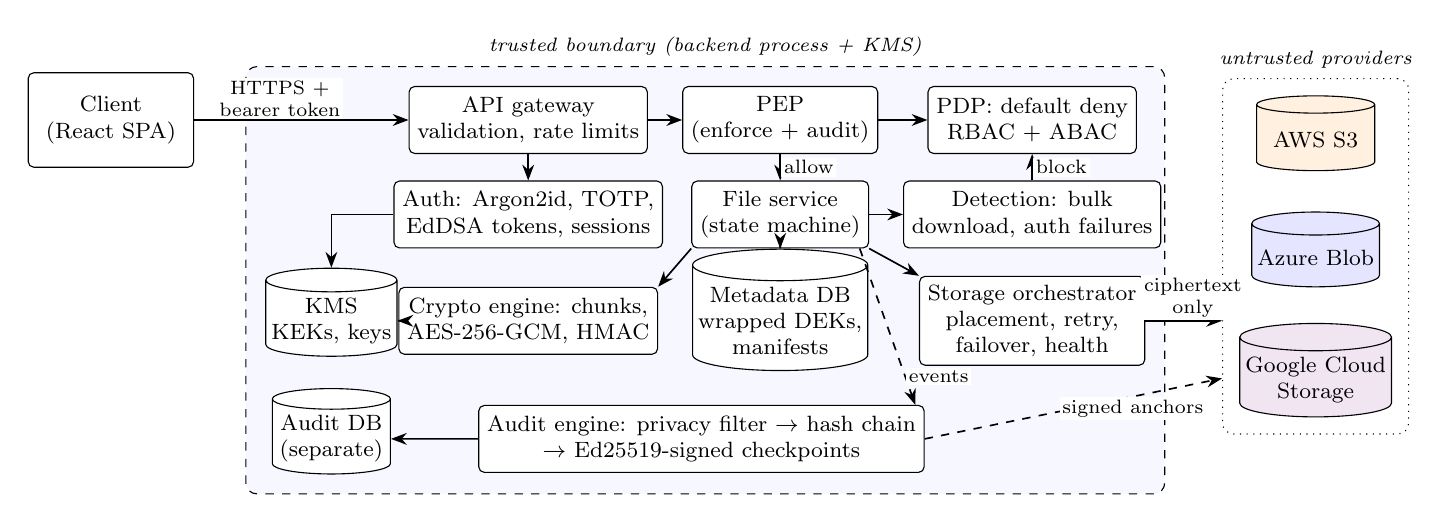
\begin{tikzpicture}[
  font=\footnotesize,
  box/.style={draw, rounded corners=2pt, align=center, minimum height=0.85cm, minimum width=2.6cm, inner sep=3pt, fill=white},
  store/.style={draw, cylinder, shape border rotate=90, aspect=0.18, align=center, minimum height=0.95cm, minimum width=1.5cm, inner sep=2pt, fill=white},
  arr/.style={-{Stealth[length=2mm]}, semithick},
  darr/.style={-{Stealth[length=2mm]}, semithick, dashed},
  lab/.style={font=\scriptsize, fill=white, inner sep=1pt}
]
\node[box, minimum width=2.1cm, minimum height=1.2cm] (client) at (-1.9,1.2) {Client\\(React SPA)};
\node[box] (api)   at (3.4,1.2)  {API gateway\\validation, rate limits};
\node[box, minimum width=2.1cm] (pep) at (6.6,1.2) {PEP\\(enforce + audit)};
\node[box] (pdp)   at (9.8,1.2)  {PDP: default deny\\RBAC + ABAC};
\node[box] (auth)  at (3.4,0)    {Auth: Argon2id, TOTP,\\EdDSA tokens, sessions};
\node[box, minimum width=2.1cm] (files) at (6.6,0) {File service\\(state machine)};
\node[box] (det)   at (9.8,0)    {Detection: bulk\\download, auth failures};
\node[store] (kms) at (0.9,-1.35) {KMS\\KEKs, keys};
\node[box] (crypto) at (3.4,-1.35) {Crypto engine: chunks,\\AES-256-GCM, HMAC};
\node[store] (mdb) at (6.6,-1.35) {Metadata DB\\wrapped DEKs,\\manifests};
\node[box] (orch)  at (9.8,-1.35) {Storage orchestrator\\placement, retry,\\failover, health};
\node[store] (adb) at (0.9,-2.85) {Audit DB\\(separate)};
\node[box, minimum width=5.0cm] (audit) at (5.6,-2.85) {Audit engine: privacy filter $\rightarrow$ hash chain\\$\rightarrow$ Ed25519-signed checkpoints};
\begin{scope}[on background layer]
\node[draw, dashed, rounded corners=4pt, fill=blue!3, fit=(api)(pdp)(kms)(adb)(audit)(orch), inner sep=7pt,
      label={[font=\scriptsize\itshape]above:trusted boundary (backend process + KMS)}] (tb) {};
\end{scope}
\node[store, fill=orange!12] (s3) at (13.4,0.95) {AWS S3};
\node[store, fill=blue!10]   (az) at (13.4,-0.55) {Azure Blob};
\node[store, fill=violet!10] (gcs) at (13.4,-2.1) {Google Cloud\\Storage};
\begin{scope}[on background layer]
\node[draw, dotted, rounded corners=4pt, fit=(s3)(gcs), inner sep=6pt,
      label={[font=\scriptsize\itshape]above:untrusted providers}] (prov) {};
\end{scope}
\draw[arr] (client.east) -- node[lab, above, pos=0.4, align=center] {HTTPS +\\bearer token} (api.west);
\draw[arr] (api) -- (pep);
\draw[arr] (pep) -- (pdp);
\draw[arr] (api) -- (auth);
\draw[arr] (pep) -- node[lab, right] {allow} (files);
\draw[arr] (files) -- (det);
\draw[arr] (det) -- node[lab, right] {block} (pdp);
\draw[arr] (auth.west) -| (kms.north);
\draw[arr] (crypto.west) -- (kms.east);
\draw[arr] (files.south west) -- (crypto.north east);
\draw[arr] (files) -- (mdb);
\draw[arr] (files.south east) -- (orch.north west);
\draw[darr] ($(files.south east)+(-0.12,0)$) -- node[lab, right, pos=0.82] {events} ($(audit.north east)+(-0.12,0)$);
\draw[arr] (audit.west) -- (adb.east);
\draw[arr] (orch.east) -- node[lab, above, pos=0.62, align=center] {ciphertext\\only} (orch.east -| prov.west);
\draw[darr] (audit.east) -- node[lab, below, pos=0.7] {signed anchors} ($(prov.west)+(0,-1.55)$);
\end{tikzpicture}
\caption{Architecture. Solid arrows are data or control flow; every component emits audit events (shown for the file service). The dashed box is the trusted boundary. Providers receive only ciphertext under opaque names and signed audit checkpoints (anchors). The policy decision always precedes key unwrapping.}
\label{fig:arch}
\end{figure*}

\subsection{Identity and per-request zero-trust policy}
\textbf{Authentication.} Passwords are hashed with Argon2id (time cost 3, 64\,MiB, parallelism 4 by default)~\cite{rfc9106}. TOTP~\cite{rfc6238} seeds are stored encrypted by the KMS. Five consecutive failures lock an account for 15 minutes, and wrong TOTP codes count towards the same limit. Access tokens are EdDSA-signed JWTs with a 5-minute lifetime. They carry only identifiers and standard claims, and the algorithm is pinned so that \code{alg:none} and HS256 confusion are refused. Refresh tokens are 256-bit random values sent in an \code{HttpOnly}, \code{SameSite=Strict} cookie. They are stored only as an HMAC, are single-use and rotate on every refresh. Presenting a used refresh token is treated as theft and revokes the whole session. Sessions have a 30-minute idle and a 12-hour absolute lifetime.

\textbf{Per-request policy.} A PEP wraps every sensitive operation. It loads the resource, re-reads the user (role, active flag, allow list) and the session from the database, and calls a pure PDP with \emph{(subject, action, resource, context)}. No authorisation data is trusted from the token, so revocation, disablement and role changes take effect on the next request. The PDP combines RBAC (roles \emph{user}, \emph{auditor}, \emph{admin}) with attribute rules: ownership or an explicit share; clearance at least the file's classification (public $<$ internal $<$ confidential $<$ restricted); MFA verified within 10 minutes for delete, share, administrative actions and reads of confidential or higher files; source IP within the user's CIDR allow list; and no active block from the download-anomaly detector. The detector blocks a subject after 20 downloads or 512\,MiB within 5 minutes by default. The default is deny, and every decision is audited with reason codes. Unknown and unauthorised file IDs both return \code{404}, so guessing reveals nothing. Administrators manage users, keys and policy, but a separation-of-duties rule (\code{admin-no-content-access}) denies them any read, delete or share of other users' files.

\subsection{Chunking and cryptography}
Algorithm~\ref{alg:upload} summarises the upload path. Each file receives a fresh 256-bit DEK from the KMS. The DEK is wrapped with AES-256-GCM under a versioned KEK, with the wrap bound to \{file id, owner id\} as associated data. A wrapped key copied to another row, or a file whose owner is changed in the database, therefore fails to unwrap. HKDF-SHA256~\cite{rfc5869} derives three independent keys from the DEK, labelled \code{chunk-encryption}, \code{manifest-mac} and \code{metadata-encryption}. The file is streamed in 1\,MiB chunks by default. The chunk size is a deployment setting, and each manifest records the size used for its file, so files written under different settings stay readable. Each chunk is stored as $\text{nonce}_{12}\,\|\,\text{AES-256-GCM}(m_i)$ with associated data
\begin{equation}
\mathit{AAD}_i = \texttt{"ZTC"}\,\|\,v\,\|\,\ell(\mathit{fid})\,\|\,\mathit{fid}\,\|\,i\,\|\,\mathit{final}_i ,
\end{equation}
a fixed-width, length-prefixed encoding of format version, file id, chunk index and a final-chunk flag. A chunk cannot be moved to another position or file, and the last chunk cannot be dropped, without failing authentication.

The filename and MIME type are encrypted under the metadata key. The \emph{manifest} is canonical JSON containing the file and owner ids, sizes, the ordered chunk list with ciphertext SHA-256 values, replica locations, the classification and the whole-file plaintext SHA-256. It is sealed with HMAC-SHA256 under the manifest key and is the only source of truth for reconstruction; the relational chunk tables are a projection used by the user interface. Downloads are \emph{verify-then-release}. The manifest MAC is checked before any chunk is fetched; each chunk's SHA-256 and GCM tag are verified; then the whole-file hash and size are checked, and only then is plaintext streamed to the client. A corrupted file is never partially delivered. Deleting a file removes the wrapped DEK and the manifest in the same transaction (\emph{crypto-shredding}), so the data is unrecoverable even if a provider deletion fails.

\begin{algorithm}[t]
\caption{Upload (simplified)}
\label{alg:upload}
\small
\begin{algorithmic}[1]
\Require token $t$, stream $F$, classification $c$
\State $(s,u)\gets$ \textsc{Authenticate}$(t)$; re-read session and user
\If{\textsc{PDP}$(u,\texttt{file:create},c,\mathit{ctx})=\mathsf{deny}$} \State audit; \Return 403 \EndIf
\State $\mathit{fid}\gets$ random 128-bit id; state $\gets$ \textsc{Uploading}
\State $(\mathit{DEK}, W)\gets$ \textsc{KMS.GenerateDataKey}$(\{\mathit{fid},u\})$
\State $k_c,k_m,k_n\gets$ \textsc{HKDF}$(\mathit{DEK},\{\text{labels}\},\mathit{fid})$
\For{each chunk $m_i$ of $F$ (1\,MiB)}
  \State $b_i\gets \nu_i\,\|\,\textsc{GCM}_{k_c}(\nu_i, m_i, \mathit{AAD}_i)$
  \State $P_i\gets$ \textsc{Placement}$(\mathit{fid}, i)$ \Comment{$R{=}2$ of 3, rotating}
  \State \textsc{Orchestrator.Put}$(\text{opaque id}, b_i, P_i)$ \Comment{retry, failover, read-back}
\EndFor
\State $M\gets$ manifest$(\mathit{fid},u,\{\mathrm{SHA256}(b_i)\},P,c,\mathrm{SHA256}(F))$
\State store $W$, $M$, $\textsc{HMAC}_{k_m}(M)$, $\textsc{GCM}_{k_n}(\text{name})$; state $\gets$ \textsc{Committed}
\State audit \texttt{file.upload}; erase $\mathit{DEK}$
\Statex \emph{On any failure: state $\gets$ \textsc{Failed}, stored chunks deleted, $W$ discarded.}
\end{algorithmic}
\end{algorithm}

\subsection{Multi-cloud placement and resilience}\label{sec:placement}
Three provider adapters (AWS S3, Azure Blob, Google Cloud Storage) implement one storage interface. Each chunk is written to $R=2$ distinct providers chosen by a rotating placement: the starting provider is derived from $\mathrm{SHA\text{-}256}(\mathit{fid}) \bmod n$ and advances per chunk, and the remaining providers are ordered fallbacks. An upload commits only if every chunk reached the minimum number of write replicas (default 2). If a target is unhealthy, the orchestrator fails over to another provider. Writes are verified by a \code{stat} and a read-back SHA-256 comparison. Calls are retried with bounded exponential backoff and full jitter: at most 4 attempts, with the delay before retry $k$ drawn uniformly from $[0,\min(3\,\mathrm{s}, 0.2\,\mathrm{s}\cdot 2^{k-1})]$. A per-provider circuit breaker opens after 3 consecutive failures for a 30\,s cool-down and then admits a single half-open trial. Health is also probed in the background. On read, a replica that is missing, unavailable or whose SHA-256 differs from the manifest is skipped in favour of the other replica and recorded as a critical audit event. A \emph{verify} (scrub) operation checks every replica without decrypting, and \emph{repair} re-replicates from an intact copy and re-seals the manifest.

\emph{Honest note.} This is replication, not erasure coding or secret sharing~\cite{rabin1989,shamir1979,bessani2011depsky}. With $R=2$ of 3, each provider holds about two-thirds of the ciphertext chunks. Confidentiality against providers rests on encryption, not on dispersal. Losing both replicas of a chunk makes the file unavailable (reported as \code{503 data-unavailable}, never as wrong bytes). Setting $R=1$ maximises dispersal at the cost of all fault tolerance.

\subsection{Privacy-aware tamper-evident audit}
Every record stores $h_n = \mathrm{SHA\text{-}256}(h_{n-1}\,\|\,\mathrm{canonical}(r_n))$ with a strictly increasing sequence number, and appends are serialised. Every 100 events (and on demand) an Ed25519-signed checkpoint $\{\mathit{seq}, h_{\mathit{seq}}, \mathit{time}\}$ is written to the audit database \emph{and} uploaded as an \emph{anchor} to all three providers. Anchors live in a per-log namespace \code{anchors/audit/<log\_id>/}, where \code{log\_id} is derived from the audit-signing public key, so deployments sharing a bucket cannot overwrite each other's evidence. The audit log uses its own database, separate from the metadata database.

Privacy controls apply before a record is hashed. Actors appear only as keyed pseudonyms, $\texttt{u\_}\|\mathrm{HMAC}_{k_p}(\mathit{uid})$ truncated to 16 bytes. Event details pass through a per-event-type allow-list of field names and a deny-pattern scan for secrets. Source IPs are generalised to /24 (IPv4) or /48 (IPv6). Filenames, usernames, tokens, keys and content never enter the log. Users see their own events and auditors see all events by pseudonym. Mapping a pseudonym back to an account requires an admin with fresh MFA and is itself audited (\code{audit.reidentify}). Retention (365 days by default) deletes only whole prefixes that end at a newly signed retention checkpoint, which becomes the verifiable starting point. These controls matter because investigation depends on the log: the published threat-hunting guidance for this campaign relies on historical access logs~\cite{mandiant2024hunting}. A per-request audit context (request id, actor pseudonym, source network) is propagated through \code{contextvars} into the storage thread pools, so a storage integrity alert can be joined to the request and user that triggered it.

\subsection{MFA enrolment under credential theft}\label{sec:tofu}
MFA is the control the case study identifies as decisive~\cite{casestudy2026}, but enrolling a factor is itself an authentication problem. Suppose a user has not yet enrolled. A session that has proved only the password cannot be distinguished from a thief holding that password. If such a session may enrol a factor, the thief enrols \emph{their own} authenticator. In our first implementation, activation also marked the enrolling session as MFA-verified and revoked all other sessions. The thief thus gained step-up rights and locked the real owner out behind a factor only the thief held (finding F1, Section~\ref{sec:findings}). Requiring MFA at sign-in does not help, because restricted sessions must be able to reach enrolment.

Our design (ADR-0010) rests on two rules. \emph{(1) Activation grants nothing.} Activating a factor neither marks the current session MFA-verified nor revokes other sessions; verified status comes only from a new login with the code or an explicit step-up. Activation is audited at WARNING with the source network. \emph{(2) Who may establish a first factor.} Without approval, only (a)~an account that never had a factor, within 24\,h of registration (trust on first use, when the password is newest and least likely to be stolen), or (b)~the bootstrap administrator while no other administrator holds a factor. Anyone else needs a single-use, user-bound, 24-hour enrolment code issued by an administrator with fresh MFA. Only an HMAC of the code is stored. Replacing a factor requires a code from the current one, and the self-enrolment window never reopens once an account has had a factor. MFA at sign-in is on by default, and a password-only session can reach only \code{/me}, logout, refresh, gated enrolment and the policy view.

The design has a stated residual risk: a password stolen \emph{inside} the 24-hour window, before the owner enrols, still lets the thief enrol and step up. This is detected (WARNING events with the thief's network) and recoverable (admin MFA reset), but not prevented. A dedicated test demonstrates it. Closing it fully requires an out-of-band channel at registration, which the system does not have. We believe this tension between usability and the first-factor bootstrap deserves more attention than it receives, because ``enable MFA'' is the standard advice after incidents such as UNC5537~\cite{cisa2024,snowflake-mfa-rollout}.

%=====================================================================
\section{Implementation}
%=====================================================================
% NUMBERS: line counts measured on 2026-11-23 with find ... | xargs wc -l
The backend is Python with FastAPI, SQLAlchemy~2 (SQLite by default, PostgreSQL by URL), the \code{cryptography} library (AES-GCM, HKDF, HMAC, Ed25519), \code{argon2-cffi} and \code{pyotp}. The provider adapters use the official SDKs: \code{boto3}, \code{azure-storage-blob} and \code{google-cloud-storage}. The KMS abstraction has a local keystore backend (entries encrypted under a 32-byte root key; production startup refuses to run without one) and an AWS KMS backend. The frontend is a React single-page application in TypeScript built with Vite. For local testing the three clouds are replaced by emulators that speak their APIs (moto server for S3, Azurite for Azure Blob, \code{gcp-storage-emulator} for GCS). The \emph{real SDK adapters} run against them unchanged. The code base comprises 14,134 lines of Python in 70 files under \code{backend/app}, 11,850 lines in 77 test files, and 4,698 lines of TypeScript/TSX/CSS under \code{frontend/src}. Twelve architecture decision records (ADR-0001 to ADR-0012) document the design choices. The container deployment overrides three framework defaults (16\,MiB chunks, a 10\,GiB upload cap and a 20\,GiB bulk-download threshold; ADR-0012), and the benchmark and large-file tools are in \code{scripts/bench/}. Fig.~\ref{fig:shots} shows two views of the user interface.

\begin{figure}[t]
\centering
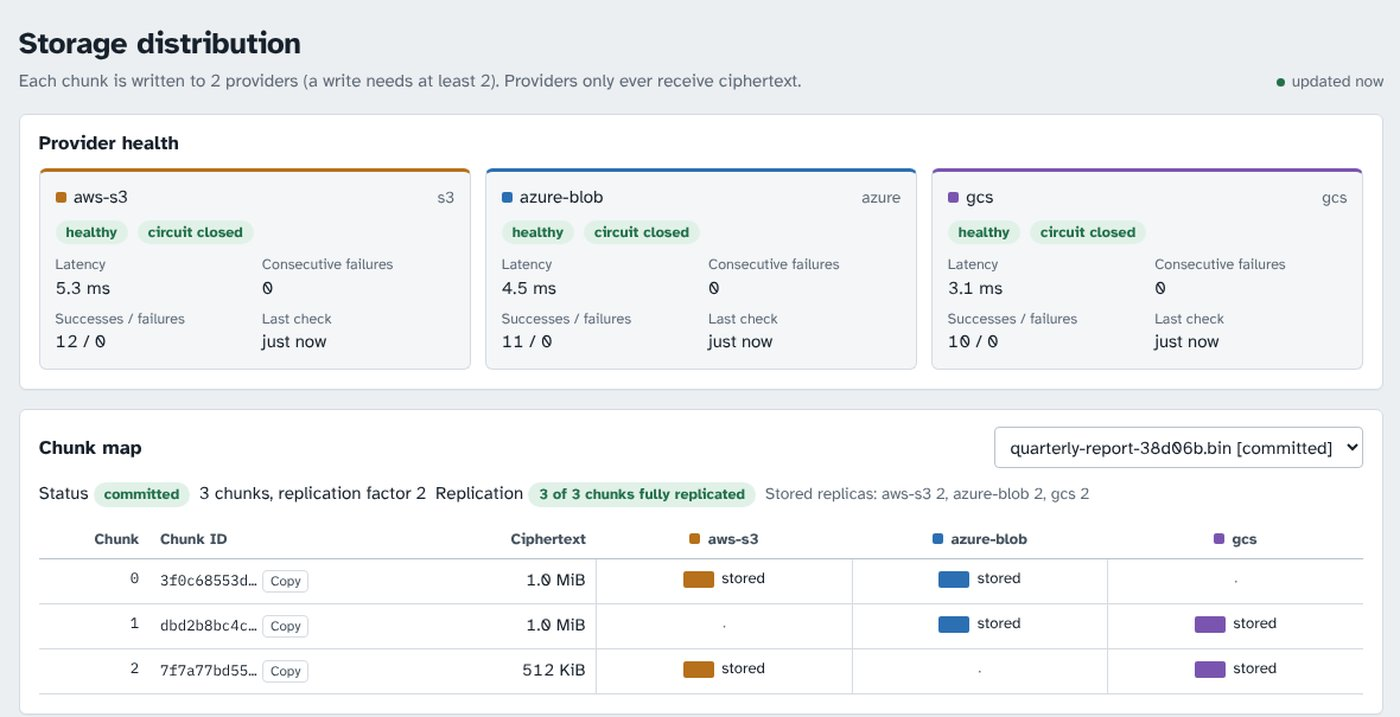
\includegraphics[width=0.9\columnwidth]{figures/distribution.jpg}\\[2pt]
{\footnotesize (a) Storage distribution: provider health and chunk map ($R=2$ of 3).}\\[4pt]
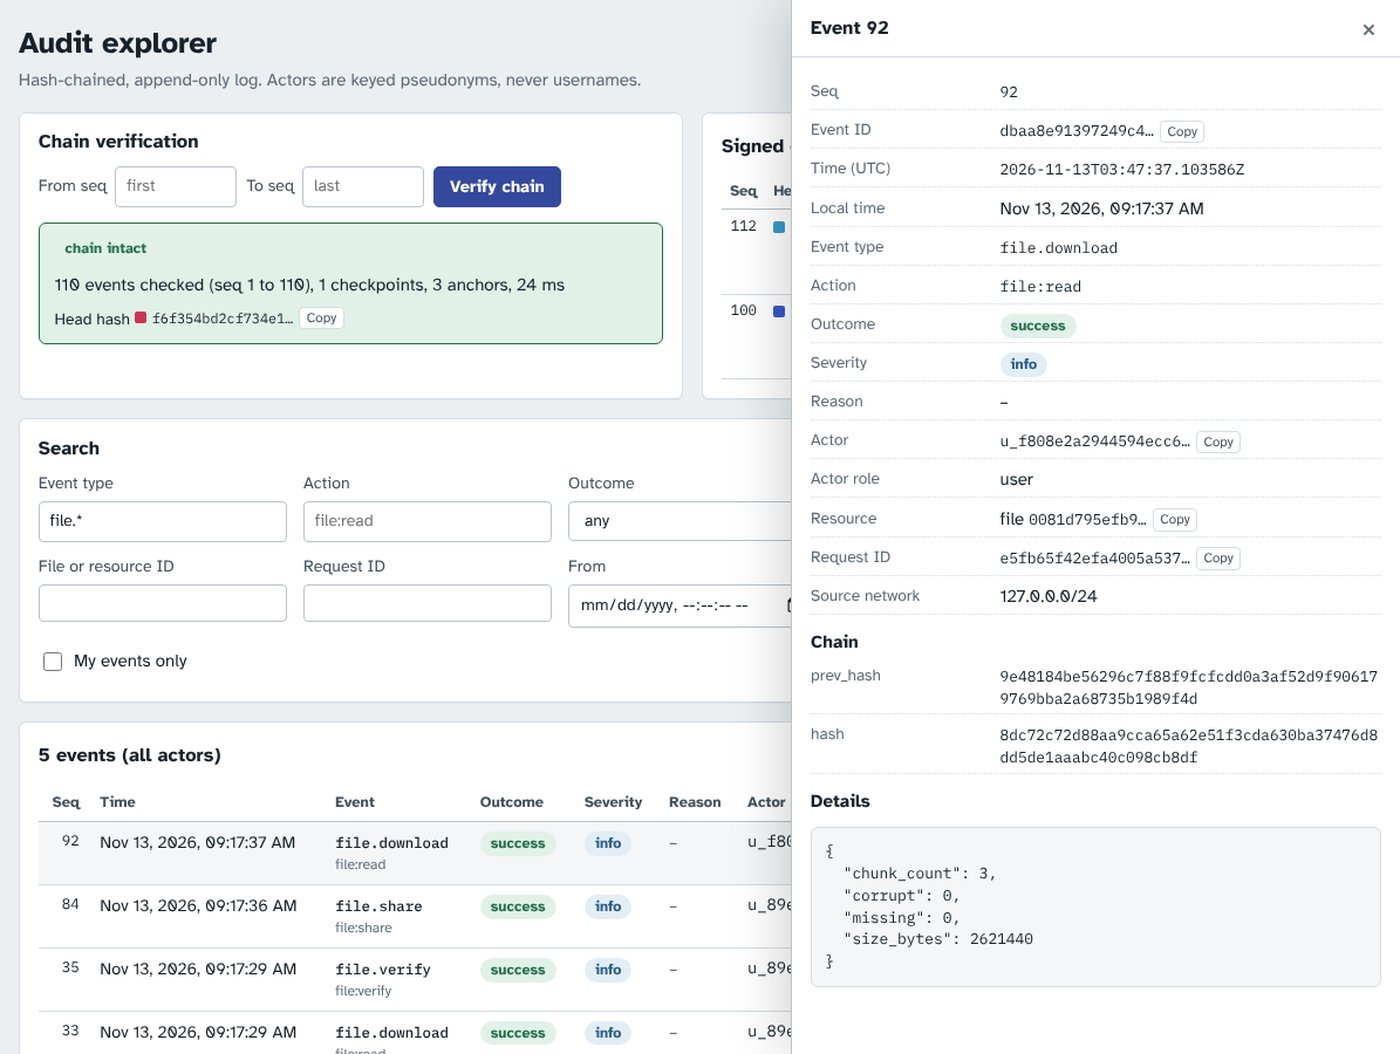
\includegraphics[width=0.9\columnwidth]{figures/audit-verify.jpg}\\[2pt]
{\footnotesize (b) Audit explorer: chain verification and an event with pseudonymous actor, /24 network and hash links.}
\caption{Screenshots of the prototype's web interface.}
\label{fig:shots}
\end{figure}

%=====================================================================
\section{Evaluation}
%=====================================================================
All experiments ran on a single host against emulators; Section~\ref{sec:limits} discusses what this does and does not show.

\subsection{Functional and test results}
Table~\ref{tab:tests} lists the recorded test runs. The security suite drives the real application container (LocalKMS, crypto engine, orchestrator, audit, authentication, PDP/PEP, detection) through a FastAPI \code{TestClient} with an injected clock and fault-injecting in-memory providers. The emulator scenarios use the real SDK adapters. Every attack test joins the HTTP response to the audit record it produced through a per-request id, so each result is an observed behaviour, not an assumption.

\begin{table}[t]
\caption{Recorded test results}
\label{tab:tests}
\centering
\footnotesize
% NUMBERS: final verification run of 2026-11-25 (docs/SECURITY_TESTING.md, docs/FINAL_REPORT.md); the Playwright row is from 2026-11-23 (not re-run).
% row 5 from backend/app/audit/NOTES.md.
\begin{tabularx}{\columnwidth}{@{}Lr@{}}
\toprule
Suite & Result \\
\midrule
Whole backend suite (\code{pytest}) & 1,273 passed \\
\quad of which security suite (S01--S17, E01--E07) & 108 passed \\
\quad of which independent-review regressions & 42 passed \\
Frontend: Vitest unit / Playwright end-to-end checks$^{*}$ & 15 / 54 of 54 \\
End-to-end demonstration over HTTP + emulators & 46 of 46 checks \\
\bottomrule
\end{tabularx}
\end{table}

The final verification run was recorded on 25 November 2026 with all three emulators reachable: 1,273 backend tests (968 unit, 155 integration, 108 security, 42 review) passed with no failures, no skips and no expected failures. $^{*}$The Playwright walk-through was last run on 23 November and was not repeated, because no browser was available for the second run; the 37 tests added since then cover the deployment settings, per-file chunk sizes and the benchmark tooling, and no application code changed. Before the fixes, the Phase-8 security suite recorded 98 passed and 8 strict \emph{xfail} tests, one per open weakness; these turned into ordinary passing tests when the weaknesses were fixed, and the 42 review tests reproduce each independent-review finding (Section~\ref{sec:findings}) against the fixed code.

\subsection{Attack scenarios}
Table~\ref{tab:attacks} summarises the 17 attack scenarios. S11--S15 replay the UNC5537 kill chain stage by stage. Documented residual risks are tested as explicit ``stated limit'' cases.

\begin{table*}[t]
\caption{Attack scenarios S01--S17 (from \code{docs/SECURITY\_TESTING.md}); every row passed}
\label{tab:attacks}
\centering
\footnotesize
% NUMBERS: observed values (41/41, 12 of 16, 109 DBs / 2,790 events / 629+65+6 secrets) from docs/SECURITY_TESTING.md Sec. 5
\begin{tabularx}{\textwidth}{@{}P{0.5cm}P{4.1cm}P{5.1cm}L@{}}
\toprule
\# & Attack & Mechanism & Observed result \\
\midrule
S01 & Forged tokens: \code{alg:none}/HS256, edited payload, foreign issuer, audience or key & EdDSA pinned; signature, \code{iss}, \code{aud} checks & 401; each attempt audited with a specific reason \\
S02 & Expired token, idle or absolute session expiry & Strict \code{exp}; session row re-read per request & 401 (session expiries audited) \\
S03 & Another user's file; 40 random ids + 1 real id & Ownership/share check; unknown = unauthorised = 404 & 41/41 guesses 404; every guess an audited deny \\
S04 & Admin reads user file; user/auditor call 9 admin ops & Separation of duties; RBAC default deny & 403 \code{admin-no-content-access} / \code{default-deny} \\
S05 & Bit flip in one / both replicas at a provider & Per-replica SHA-256 vs.\ sealed manifest; failover & One: 200, identical bytes, critical alert; both: 409, no bytes \\
S06 & Edit manifest, owner id or projection rows in metadata DB & Manifest HMAC; DEK wrap bound to (file, owner) & 409 \code{manifest-mac-invalid} / \code{key-unwrap-failed}; projection ignored \\
S07 & Reorder, substitute, truncate chunks (incl.\ forged manifest) & AAD binds version, file, index, final flag & 409 \code{chunk-auth-failed}; deleted last chunk: 503, never a short file \\
S08 & Modify, delete, reorder, truncate audit records & Hash chain, signed checkpoints, provider anchors & Detected (Table~\ref{tab:audit}); no API path edits records \\
S09 & One provider credential: read, overwrite, delete all & Ciphertext only, opaque ids; $R=2$ & 12 of 16 objects, entropy $>7.5$ bit/byte, no keys/metadata; all files still download \\
S10 & Stuffing, lockout, login flood, TOTP brute force, enumeration & Lockout (5/15\,min), rate limits, anomaly detector & Locked even with correct password; 429s audited; uniform 202 on registration \\
S11 & \textbf{UNC5537}: stolen password, with/without MFA; enrolment hijack & MFA at sign-in; step-up; ADR-0010 gating & Enrol refused outside window; no step-up from activation; TOFU limit demonstrated \\
S12 & \textbf{UNC5537}: valid credentials from outside allow list & CIDR check on login, refresh, account routes, PDP & 401 at login/refresh; 403 \code{network-not-allowed}, no lockout increment \\
S13 & \textbf{UNC5537}: bulk export by a valid session & Download count and byte thresholds $\rightarrow$ block & 403 \code{download-rate-exceeded}; critical anomaly event \\
S14 & \textbf{UNC5537}: stolen refresh token & Single-use rotation; reuse revokes the session & Thief's tokens dead after the next legitimate refresh; critical event \\
S15 & Revocation, disablement, demotion & User and session re-read per request & Effective on the next request (401) \\
S16 & Path traversal, header/markup injection, oversize, malformed ids & Filenames never paths; strict id regex; body caps & Display names only; 413/422/404, never 500 \\
S17 & Steal every audit DB and search it for secrets & Allow-list, deny scan, pseudonyms, /24 & 109 DBs, 2,790 events, 629 secrets + 65 TOTP codes + 6 IPs: 0 hits \\
\bottomrule
\end{tabularx}
\end{table*}

\subsection{Provider failures and a real outage}
Seven failure scenarios (E01--E07) ran against moto, Azurite and \code{gcp-storage-emulator} through the real adapters. They covered a killed emulator process, objects deleted or overwritten through each SDK, injected timeouts and transient failures over the real adapter, a chunk lost at every provider, and repair after a provider returns. All passed. Timeouts were retried and then failed over; two transient failures were absorbed by retries on the same provider; a chunk missing everywhere gave \code{503}, never partial content; and repair restored replication once the provider returned.

% NUMBERS: from docs/demo-output.txt steps 11, 13, 14
The end-to-end demonstration (\code{docs/demo-output.txt}) stops the GCS emulator process, a real outage rather than an injected fault. The owner's download still succeeds with byte-identical content (0.1\,s including retries). Provider health reports GCS unhealthy with a connection error. A new upload during the outage places its chunks on AWS S3 and Azure only. After the emulator restarts, health recovers and verification reports all 8 replicas intact. In the same run, one byte flipped in one Azure replica was found by the scrub without decryption (7 ok, 1 corrupt). The download remained byte-identical, a critical \code{storage.replica.corrupt} event was recorded, and repair restored a healthy state.

\subsection{What a provider sees}
% NUMBERS: from docs/demo-output.txt steps 5-8
In the demonstration a 3,670,102-byte file is split into 4 chunks (three of 1\,MiB and one smaller), each stored on 2 of the 3 providers. In this run S3 and Azure held 3 replicas each and GCS held 2; no provider held all chunks. Reading the raw objects directly with each SDK, as a holder of a provider credential would, shows opaque 32-hex-character names, an empirical entropy of 8.000 bits per byte for every object, and empty object metadata (no owner, filename or key id). No object contains the plaintext marker, the filename or the username. The ciphertext overhead is exactly 112 bytes, i.e., 28 bytes per chunk (12-byte nonce + 16-byte tag). A provider still learns object count, approximate sizes and access timing, which is non-goal~(iv).

\subsection{Audit tampering detection}
Table~\ref{tab:audit} shows what the verifier reports for each manipulation made directly in the audit database (S08). In the demonstration, an \code{UPDATE} that turned an auditor's denied access into \code{success} was reported as \code{record-modified} at that sequence number. The check covered 64 events, 2 checkpoints and 6 anchors, and the verification run was itself audited as critical. The stated limit is that records written after the last anchored checkpoint can be deleted or consistently rewritten without detection until the next checkpoint (a window of \code{audit\_checkpoint\_every} = 100 events by default). An attacker who controls the audit database, the audit-signing key and every anchor copy can rewrite history.

\begin{table}[t]
\caption{Audit tampering detection (S08)}
\label{tab:audit}
\centering
\footnotesize
\begin{tabularx}{\columnwidth}{@{}P{2.9cm}L@{}}
\toprule
Manipulation (direct SQL) & Verifier findings \\
\midrule
Modify a record & \code{record-modified} \\
Modify and recompute its hash & \code{chain-broken} \\
Delete a record & \code{chain-broken}, \code{sequence-gap} \\
Swap two records & \code{chain-broken}, \code{record-modified}, \code{reordered} \\
Truncate covered tail & \code{truncated} \\
Truncate tail and all checkpoint rows & \code{checkpoint-missing}, \code{truncated} (via anchors) \\
Rewrite a checkpoint row & \code{checkpoint-signature-invalid}, \code{anchor-mismatch} \\
Delete events after last checkpoint & \emph{not detected} (stated limit) \\
\bottomrule
\end{tabularx}
\end{table}

\subsection{Performance}\label{sec:perf}
% NUMBERS: audit numbers from backend/app/audit/NOTES.md ("Measured performance"); end-to-end numbers: see Section~\ref{sec:stats} (analysis/data via analysis/run_all.sh).
The audit subsystem's own measurements (\code{backend/app/audit/NOTES.md}) are as follows. 1,000 real \code{record()} calls take 1.35\,s, i.e., about 739 events/s with an fsync per event. Verifying a chain of 20,000 events with 190 signed checkpoints and 570 anchor copies takes 0.54\,s. The end-to-end figures below were measured through the full API stack (authentication, PDP, KMS, encryption, $R=2$ placement with read-back verification, audit) against the three emulators; they exclude network latency, so they show the cost of the security pipeline and of per-chunk work, not achievable cloud throughput. A download is verified in full before its first byte is released (the plaintext is held in memory up to 8\,MiB and in a temporary file beyond that), so its latency grows with file size by design.

\subsection{Statistical evaluation}\label{sec:stats}
% NUMBERS: analysis/data/*.csv through analysis/analyze.py (docs/STATISTICAL_ANALYSIS.md); reproduce with analysis/run_all.sh.
We measured the framework with the scripts in \code{analysis/}; one command reproduces every number. Each API measurement is one request to a real server on the loopback interface, with conditions interleaved in random order, $n=30$ repetitions per condition after three discarded warm-ups, and 95\% confidence intervals. Two groups are compared with Welch's $t$-test, or the Mann--Whitney $U$ test when a Shapiro--Wilk test rejects normality; several groups with Kruskal--Wallis; proportions with Wilson intervals; placement and ciphertext with $\chi^2$ tests. The host is an Intel(R) Core(TM) Ultra 9 185H (22 logical CPUs, 15.3\,GiB) under WSL2, Python 3.12.3, commit \code{511eb14}; absolute times belong to this machine, ratios and shapes are the transferable part. Table~\ref{tab:stats} and Figs.~\ref{fig:statmain} and~\ref{fig:stataux} summarise the results.

\begin{table}[t]
\caption{Key results of the statistical evaluation (95\% confidence intervals in brackets)}
\label{tab:stats}
\centering
\footnotesize
\begin{tabularx}{\columnwidth}{@{}>{\raggedright\arraybackslash}p{2.35cm}L@{}}
\toprule
Question & Result \\
\midrule
Scaling (a) & Time grows roughly linearly with size: upload 5.9\,MiB/s [5.5, 6.4], download 61.5\,MiB/s [56.1, 68.1]; $R^2$ 0.869 and 0.782. \\
Cost of security (b), 16\,MiB & Full pipeline against plain chunked storage of the same bytes: upload $\times$1.15 ($+$0.50\,s [0.04, 0.97], Mann-Whitney U, $p=0.008$), download $\times$3.40. AES-256-GCM with SHA-256 explains 3\% of the upload and 5\% of the download difference. \\
Chunk size (c) & Throughput depends on chunk size (Kruskal--Wallis, upload $p<0.0001$, download $p<0.0001$); median upload 1.4\,MiB/s at 256\,KiB and 32.4\,MiB/s at 16\,MiB. \\
One provider killed (d) & 100/100 reads and 100/100 writes succeed (Wilson lower bounds 96.3\% and 96.3\%); steady download latency $-$31.4\,ms [$-$91.2, +28.5] (no detectable change; Mann-Whitney U, $p=0.212$). Two killed: 0/10 reads. \\
Placement (e) & Replicas are uniform over the providers: rotating $\chi^2=0.01$ ($p=0.997$), hash $\chi^2=1.98$ ($p=0.373$); 2 d.f. \\
Stored objects (f) & Entropy 7.9998--7.9999 bits/byte for random, text and all-zero plaintext; the chi-square test rejected uniformity for 4 of 48 objects (8.3\%; 5\% expected by chance). \\
Audit log (g) & Verification time is linear in the log size (log-log slope 0.976 [0.961, 0.991]); 758\,events/s with an fsync per event. \\
Attack suite (h) & 108/108 designed attack and failure tests passed (Wilson lower bound 96.6\%); not a random sample. \\
Coverage (i) & 92.6\% line coverage of \code{backend/app} by the 1,273-test suite. \\
\bottomrule
\end{tabularx}
\end{table}

\begin{figure*}[t]
\centering
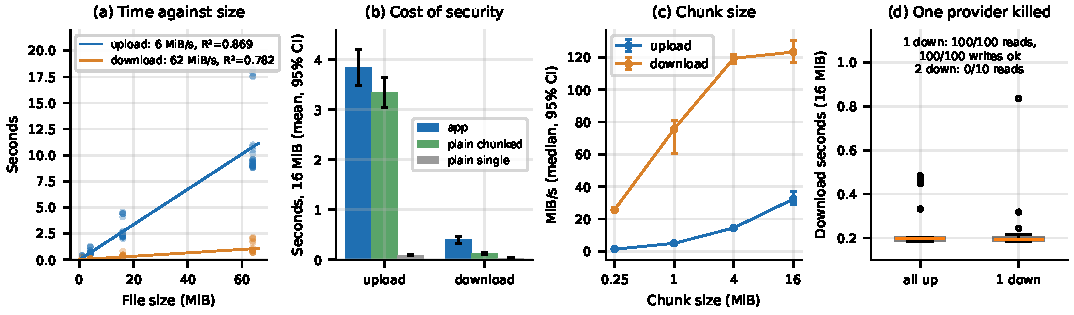
\includegraphics[width=\textwidth]{figures/stat-main.pdf}
\caption{(a) Transfer time against file size with the fitted line; (b) the same bytes stored with the full pipeline and as plain chunked and plain single-object storage; (c) throughput against chunk size for a 32\,MiB file; (d) download latency with one provider killed, and the read and write success counts.}
\label{fig:statmain}
\end{figure*}

\begin{figure*}[t]
\centering
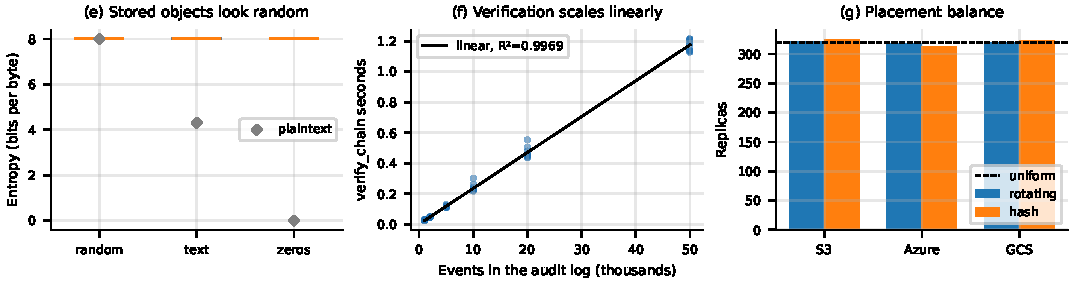
\includegraphics[width=\textwidth]{figures/stat-aux.pdf}
\caption{(e) Entropy of the objects as stored at the providers against the entropy of the plaintext; (f) audit-chain verification time against the number of events; (g) replicas per provider for the two placement strategies.}
\label{fig:stataux}
\end{figure*}

At 16\,MiB the pipeline adds 15\% to the upload time and multiplies the download time by 3.4 compared with plain chunked storage of the same bytes; the cipher itself accounts for only a few per cent of that difference, and the rest was not decomposed. Larger chunks raise throughput (uploads from 1.4 to 32.4\,MiB/s between 256\,KiB and 16\,MiB chunks). Losing one provider caused no failed request and no detectable latency change, while losing two broke every read, as the replication factor predicts. The stored objects are statistically indistinguishable from random bytes, and audit verification scales linearly. These results come from emulators on one host with no network latency, from designed (not randomly sampled) attack scenarios, and from sequential requests that are not fully independent, so they bound the cost of the pipeline rather than predict cloud performance.

%=====================================================================
\section{Security Findings and Lessons}\label{sec:findings}
%=====================================================================
We tested our own system adversarially, and the results are part of the contribution. During Phase-8 security testing, no application code was changed. Each weakness found was written as a \emph{strict xfail} test, which fails the suite as soon as the weakness is fixed and therefore cannot be forgotten. Six weaknesses were found:
\textbf{F1} (high) MFA-enrolment hijack from a password-only session (Section~\ref{sec:tofu});
\textbf{F2} (medium-high) the network allow list was enforced by the PDP but not at login, refresh and account-management endpoints, so valid credentials from outside the allow list still obtained a session and could change the password or enrol MFA;
\textbf{F3} (low) username enumeration through registration;
\textbf{F4} (medium) audit anchors were not namespaced per deployment, so two deployments sharing a bucket overwrote each other's anchors and verification reported tampering where there was none. This happened three times during testing;
\textbf{F5} (low-medium) storage-layer audit events carried no request context; and
\textbf{F6} (low) rate-limit rejections were not audited.

An independent adversarial review then reported 17 further findings: two high (H1, H2), five medium (M1--M5), eight low (L1--L8) and two informational (I1, I2). \textbf{H1}: a password change required no step-up and revoked the owner's sessions. A thief could therefore change the password and evict the owner. The fix requires a factor verified within the step-up window, refuses accounts without a factor and never revokes a session that verified MFA more recently. \textbf{H2}: with \code{X-Forwarded-For} trust enabled, only the first header line was read. Behind proxies that append a separate line, a client could choose its own IP, bypassing the allow list, evading rate limits and forging the audit network. The fix (ADR-0011) joins all header lines, takes the entry a configured number of trusted hops from the right, optionally pins trusted proxy networks, and rejects malformed chains with \code{400} instead of falling back. Medium findings included a restricted session that could still list or revoke sessions (M5), an auditor role that could map pseudonyms to usernames through the user list without the audited path (M1), single-person rotation of the pseudonym key, which would have orphaned history (M3), invalid-token floods that could push critical events out of view (M2), and an insecure default environment (M4). All 23 findings are fixed, each with a regression test.

\textbf{Lessons.}
(1)~\emph{The bootstrap of a control is part of the control.} F1, H1 and M5 are the same mistake in different places: account-management actions trusted a session that had proved only the password. That is precisely the UNC5537 attacker's position, so any action that changes how identity is proved must require the factor it protects.
(2)~\emph{Enforce a policy wherever the attribute is used, not where the policy engine happens to run.} F2 existed because the allow list was a PDP rule and the authentication endpoints never called the PDP.
(3)~\emph{Trust in infrastructure metadata is configuration-dependent.} H2 was invisible in tests without a proxy, and its impact reached the allow list, rate limiting and the audit log at once.
(4)~\emph{Privacy promises fail through side doors.} The pseudonym design was sound, but a convenience endpoint (M1) and an administrative action (M3) undermined it.
(5)~\emph{Tamper evidence needs namespacing.} F4 produced false tamper alarms, which in operation erode trust in true ones.
(6)~\emph{Make residual risks executable.} Stated limits (the TOFU window, the unanchored tail, two providers wiped) are tests, so a change in behaviour is noticed.

%=====================================================================
\section{Limitations and Future Work}\label{sec:limits}
%=====================================================================
\emph{Emulators, not clouds.} All provider results come from moto, Azurite and \code{gcp-storage-emulator} on one host. Real IAM policies, latency, eventual-consistency effects and costs were not evaluated, and no TLS or reverse proxy was in the path. The chunk-size tuning of Section~\ref{sec:stats} was measured on one host with no network latency and up to 10\,GiB; on real links a large chunk is a larger retry unit, so the 30\,s provider deadline we pair with 16\,MiB chunks should be re-validated against real providers. \emph{Single instance.} Rate limiting, lockout counters, health state and audit-append serialisation are per process; a distributed deployment needs shared state (the PostgreSQL advisory-lock path for the audit chain exists but is untested). \emph{Bearer tokens.} Access tokens are not bound to the client; DPoP~\cite{rfc9449} or mutual-TLS-bound tokens~\cite{rfc8705} would make a stolen token far less useful within its 5-minute lifetime. \emph{TOFU window.} Closing the enrolment window requires an out-of-band channel or enterprise identity federation. \emph{Erasure coding.} Reed--Solomon or IDA-style coding~\cite{rabin1989,bessani2011depsky} would lower storage overhead and give true dispersal, at the cost of complexity. \emph{Client-side encryption.} The backend sees plaintext and keys (non-goal~(ii)); end-to-end encryption in the client would remove this but complicates sharing, server-side verification and detection. \emph{HSM-backed KMS.} The local keystore should be replaced by an external KMS or HSM in production; an AWS KMS adapter exists but was exercised only against moto. Finally, timing side channels were not measured, no fuzzing beyond a hand-picked payload list was performed, and there are no React component tests.

%=====================================================================
\section{Conclusion}
%=====================================================================
The UNC5537 campaign showed that encryption cannot protect data from someone the system believes is the owner. We built a multi-cloud storage framework in which every key operation sits behind a per-request, default-deny policy decision that checks identity freshness, network, clearance and behaviour. Providers hold only context-bound ciphertext. The audit trail is tamper-evident, externally anchored and pseudonymous. The prototype passes its 17 attack scenarios and survives a real provider outage; a statistical evaluation puts the price of that protection at 15\% more upload time and 3.4 times the download time of plain chunked storage at 16\,MiB. The most instructive result came from our own testing, however. The first version repeated the incident's root cause in a new place, because a password-only session could establish the second factor. Zero trust has to cover the processes that create and change credentials as well as the requests that use them.

\section*{Acknowledgment}
The authors thank the course instructor of Cloud SRE and Security at IIIT Dharwad for guidance on the case study and the project.

\bibliographystyle{IEEEtran}
\bibliography{references}

\end{document}
